\documentclass[usenames,dvipsnames,notes]{beamer}
\usepackage{ifthen}
\usepackage{xcolor}
\usepackage{pgfplots}
\usepackage{amsmath}
\usepackage{centernot}
\usepackage{pifont}
\usepackage{tabularx}
\usepackage{makecell}
\usepackage{cuted}
\usepackage{booktabs}
\usepackage{array}

\usepackage{pgfpages}
%\setbeameroption{show notes on second screen}


\input ../beamer-style
\input ../std-macros
\input ../macros
\tikzset{vector/.style={draw,rounded corners,very thick,#1,fill=#1!15,minimum width=2cm,minimum height=1cm}}
\tikzset{vector/.default={blue}}
\tikzset{arrow/.style={draw,->,>=stealth,very thick,#1}}
\tikzset{arrow/.default={black}}
\tikzset{font={\fontsize{18pt}{12}\selectfont}}

\tikzset{state/.style={draw,circle,very thick,#1,fill=#1!15,inner sep=0pt,minimum size=1cm}}
\tikzset{state/.default={blue}}


%\hypersetup{
%    colorlinks,
%    citecolor={blue!50!black},
%    urlcolor={blue!80!black}
%}

\AtBeginSection[]
{
    \begin{frame}
        \frametitle{Table of Contents}
        \tableofcontents[currentsection]
    \end{frame}
}
\parskip=10pt

\title[CSCI-GA.2590]{Sequence Labeling}
\author[He He]{He He
}
\institute[NYU]{New York University}
\date{\today}

\begin{document}
\begin{frame}
\titlepage
\end{frame}

\section{Introduction}

\begin{frame}
    {Sequence labeling}
    Language modeling as sequence labeling:
    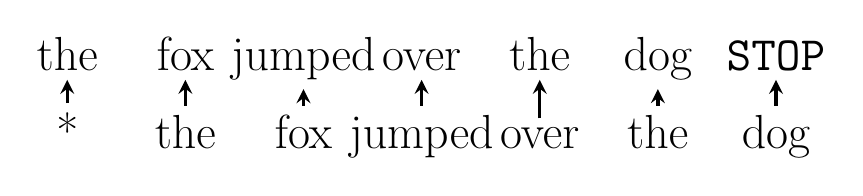
\begin{tikzpicture}
        \foreach \i\j\k in {0/*/the, 1/the/fox, 2/fox/jumped, 3/jumped/over, 4/over/the, 5/the/dog, 6/dog/\texttt{STOP}}{
            \node[anchor=base] (i\i) at (1.5*\i, 0) {\j};
            \node[anchor=base] (o\i) at (1.5*\i, 1) {\k};
            \path[draw,arrow] (i\i.north) -- (o\i.south);
        }
    \end{tikzpicture}

    \bigskip
    \textbf{Part-of-speech (POS) tagging}:
    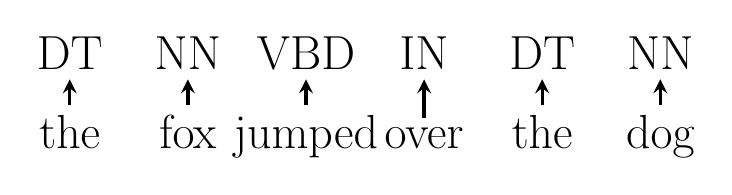
\begin{tikzpicture}
        \foreach \i\j\k in {0/the/DT, 1/fox/NN, 2/jumped/VBD, 3/over/IN, 4/the/DT, 5/dog/NN}{
            \node[anchor=base] (i\i) at (1.5*\i, 0) {\j};
            \node[anchor=base] (o\i) at (1.5*\i, 1) {\k};
            \path[draw,arrow] (i\i.north) -- (o\i.south);
        }
    \end{tikzpicture}
\end{frame}

\begin{frame}
    {Span prediction}
    \textbf{Named-entity recognition (NER)}:\\
    \vspace{2em}
    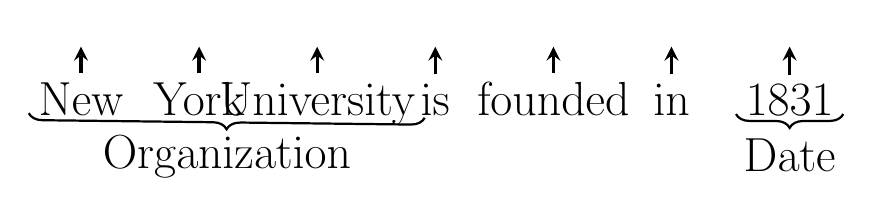
\begin{tikzpicture}
        \foreach \i\j\k in {0/New/, 1/York/, 2/University/, 3/is/, 4/founded/, 5/in/, 6/1831/}{
            \node[anchor=base] (i\i) at (1.5*\i, 0) {\j};
            \node[anchor=base] (o\i) at (1.5*\i, 1) {\k};
            \path[draw,arrow] (i\i.north) -- (o\i.south);
        }
        \path[draw,decorate,thick,decoration={brace,mirror,amplitude=5pt,raise=5pt}] (i0.west) -- (i2.east) node[midway,yshift=-20pt] {Organization};
        \path[draw,decorate,thick,decoration={brace,mirror,amplitude=5pt,raise=5pt}] (i6.west) -- (i6.east) node[midway,yshift=-20pt] {Date};
    \end{tikzpicture}

    \textbf{BIO notation}:\\
    \begin{itemize}
        \item Reduce span prediction to sequence labeling
        \item \texttt{B-<tag>}: the first word in span \texttt{<tag>}
        \item \texttt{I-<tag>}: other words in span \texttt{<tag>}
        \item \texttt{O}: words not in any span
    \end{itemize}
\end{frame}

\begin{frame}
    {POS tagging}
    \textbf{Part-of-speech}: the \emph{syntactic} role of each word in a sentence

    POS tagset:\\
    \begin{itemize}
        \item Universal dependency tagset
            \begin{itemize}
                \item \textbf{Open class tags}: content words such as nouns, verbs, adjectives, adverbs etc.
                \item \textbf{Closed class tags}: function words such as pronouns, determiners, auxiliary verbs etc. 
            \end{itemize}
        \item \href{https://www.ling.upenn.edu/courses/Fall_2003/ling001/penn_treebank_pos.html}{Penn Treebank tagset} (developed for English, 45 tags)
    \end{itemize}

    Application:\\
    \begin{itemize}
        \item Often the first step in the NLP pipeline.
        \item Used as features for other NLP tasks.
        \item Included in tools such as Stanford CoreNLP and spaCy.
    \end{itemize}
\end{frame}

\begin{frame}
    {The majority baseline}
    A dumb approach: look up each word in the dictionary and return the most common POS tag.

    \pause
    Problem: \emph{ambiguity}. Example?

    \begin{figure}
        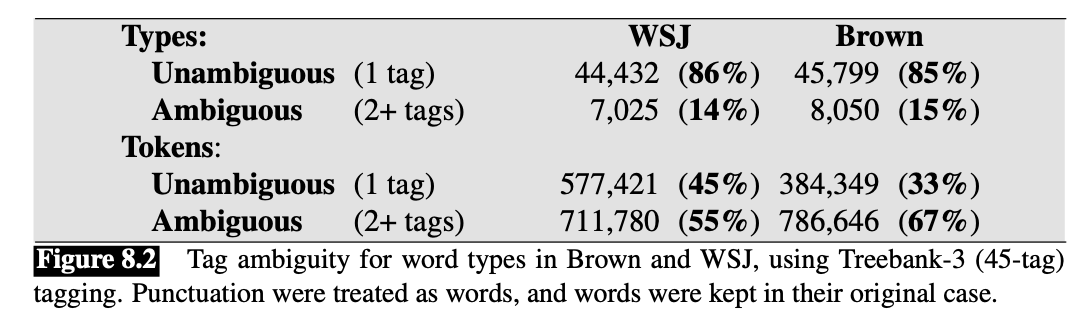
\includegraphics[height=3cm]{figures/pos-ambiguity}
    \end{figure}
    \vspace{-2em}
    Most types are unambiguous, but ambiguous ones are common words!

    Most common tag: 92\% accuracy on WSJ (vs ~97\% SOTA)\\
    \emph{Always compare to the majority class baseline.}

\end{frame}

\section{Maximum-entropy Markov Models}

\begin{frame}
    {Multiclass classifcation}
    \emph{Task}: given $x=(x_1,\ldots,x_m) \in \sX^m$, predict
    $y=(y_1,\ldots,y_m) \in \sY^m$.\\
    Predictor: $y_i=h(x, i) \quad \forall i$

    Multinomial logistic regression ($\theta\in\BR^d$):
    $$
    p(y_i\mid x) = \frac{\exp\pb{\theta\cdot\phi(x,i,y_i)}}
    {\sum_{y'\in\sY} \exp\pb{\theta\cdot\phi(x,i,y')}}
    $$

    \begin{overprint}
    \onslide<1>
    Feature templates:\\
    \vspace{8em}
    \onslide<2>
        \begin{itemize}
            \itemsep1em
            \item Learning: MLE (is the objective convex?)
            \item Inference: trivial
            \item Does not consider dependency among $y_i$'s.
                \begin{itemize}
                    \item[] \texttt{DT} \texttt{NN} ?
                    \item[] \texttt{B-<org>} \texttt{I-<org>} ?
                \end{itemize}
        \end{itemize}
    \end{overprint}
\end{frame}

\begin{frame}
    {Maximum-entropy markov model (MEMM)}
    Model the joint probability of $y_1, \ldots, y_m$:
    $$
    p(y_1,\ldots,y_m\mid x) = \prod_{i=1}^m p(y_i\mid y_{i-1}, x) \;.
    $$
    \vspace{-1em}
    \begin{itemize}
        \item Use the Markov assumption similar to n-gram LM.
        \item Insert start/end symbols: $y_0=*$ and $y_m=\texttt{STOP}$.
    \end{itemize}

    Parametrization:
    $$
    p(y_i\mid y_{i-1}, x) = \frac{\exp\pb{\theta\cdot\phi(x,i,y_i,{\color{blue}y_{i-1}})}}
    {\sum_{y'\in\sY} \exp\pb{\theta\cdot\phi(x,i,y',{\color{blue}y_{i-1}})}}
    $$

    New feature templates? (See J\&M 8.5.1)
\end{frame}

\begin{frame}
    {Inference}
    \textbf{Decoding / Inference}:
    \begin{align*}
        & \argmax_{y\in\sY^m} \prod_{i=1}^m p(y_i\mid y_{i-1}, x) \\
        &= \argmax_{y\in\sY^m} \sum_{i=1}^m \log p(y_i\mid y_{i-1}, x) \\
        &= \argmax_{y\in\sY^m} \sum_{i=1}^m \underbrace{{\color{blue}s(y_i,y_{i-1})}}_{\text{local score}} \;,
    \end{align*}
    where $s(y_i,y_{i-1}) = \theta\cdot\phi(x,i,y_i,y_{i-1})$.

    \begin{itemize}
        \item Bruteforce: exact, $O(|\sY|^m)$
        \item Greedy: inexact, $O(m)$
    \end{itemize}
\end{frame}

\begin{frame}
    {Viterbi decoding}
    %Dynamic programming:
    \vspace{-1em}
    \begin{align*}
        & \max_{y\in\sY^m} \sum_{i=1}^m s(y_i,y_{i-1}) \\
        = & \max_{y\in\sY^m} \p{ \sum_{i=1}^{m-1}s(y_i, y_{i-1}) + s(y_m, y_{m-1}) } \\
        = &\max_{{\color{blue}y_m}\in\sY} \max_{y\in\sY^{m-1}}
            \p{ \sum_{i=1}^{m-1}s(y_i, y_{i-1}) + s({\color{blue}y_m}, y_{m-1}) } \\
        = &\max_{{\color{blue}y_m}\in\sY} \max_{{\color{red}t}\in\sY} \max_{y\in\sY^{m-1},{\color{red}y_{m-1}=t}}
            \p{ \sum_{i=1}^{m-1}s(y_i, y_{i-1}) + s({\color{blue}y_m}, {\color{red}y_{m-1}=t}) } \\
        = & \max_{{\color{blue}y_m}\in\sY} \max_{{\color{red}t}\in\sY}
        \p{ s({\color{blue}y_m}, {\color{red}t}) + 
        \max_{y\in\sY^{m-1},{\color{red}y_{m-1}=t}}
        \sum_{i=1}^{m-1}s(y_i, y_{i-1}) } \\
        = & \max_{{\color{blue}y_m}\in\sY} \underbrace{
            \max_{{\color{red}t}\in\sY}
        \p{ s({\color{blue}y_m}, {\color{red}t}) + \pi[m-1, {\color{red}t}] 
        }}_{\pi[m, y_m]}
    \end{align*}
\end{frame}

\begin{frame}
    {Viterbi decoding}
    \emph{DP}: $\pi[j, t] = \max_{t'\in\sY} \pi[j-1, t'] + s(y_j=t, y_{j-1}=t')$

    \emph{Backtracking}: $p[j, t] = \argmax_{t'\in\sY} \pi[j-1, t'] + s(y_j=t, y_{j-1}=t')$

    \vspace{2em}

    %\begin{center}
    \resizebox{5cm}{!}{
    \begin{tikzpicture}
    \tikzset{font={\fontsize{18pt}{12}\selectfont}}
    \foreach \i/\w in {1/language, 2/is, 3/fun}{
        \node (s\i1) [state] at(2*\i,0) {N};
        \foreach \j/\t in {2/V, 3/A}{
            \pgfmathtruncatemacro\k{\j-1}
            \node (s\i\j) [state] [below= of s\i\k] {\t};
        }
    }
    \node (start) [state] [left=1cm of s12] {};
    \node (end) [state] [right=1cm of s32] {};

    \foreach \i in {2,...,3}{
        \pgfmathtruncatemacro\k{\i-1}
        \foreach \j in {1,...,3}{
            \foreach \t in {1,...,3}{
                \path[arrow={black!50}] (s\k\t) -- (s\i\j) ;
            }
        }
    }
    \foreach \i in {1,...,3}{
        \path[arrow={black!50}] (start) -- (s1\i);
        \path[arrow={black!50}] (s3\i) -- (end);
    }

    \foreach \i/\w in {1/language, 2/is, 3/fun}{
        \node (y\i) [above=0.3cm of s\i1] {$y_\i$};
        \node (x\i) [below=0.3cm of s\i3] {\w};
    }
    \node (ts) at(y1 -| start) {\texttt{START}};
    \node (te) at(y3 -| end) {\texttt{STOP}};

    \path[arrow={red}] ([xshift=-1ex]end.south) -- ([yshift=1ex]s33.east);
    \path[arrow={red}] ([yshift=1ex]s33.west) -- ([xshift=1ex]s22.south);
    \path[arrow={red}] ([yshift=1ex]s22.west) -- ([xshift=1ex]s11.south);
    \path[arrow={red}] ([xshift=-1ex]s11.south) -- ([yshift=1ex]start.east);

\end{tikzpicture}
}
    %\end{center}

    Time complexity?
\end{frame}

\begin{frame}
    {Viterbi decoding on the graph}
    \emph{DP}: $\pi[j, t] = \max_{t'\in\sY} \pi[j-1, t'] + s(y_j=t, y_{j-1}=t')$

    \vspace{12em}
\end{frame}

\begin{frame}
    {Summary}
    Sequence labeling: $\sX^m \rightarrow \sY^m$
    \begin{itemize}
        \item \textbf{Majority baseline}: $y_i = h(x_i)$ (no context)
        \item \textbf{Multiclass classification}: $y_i = h(x, i)$ (global input context)
        \item \textbf{MEMM}: $y_i = h(x, i, y_{i-1})$ (global input context, previous output context)
    \end{itemize}

    Problem: $y_t$ cannot be influenced by future evidence (more on this later)

    Next: score $x$ and the output $y$ instead of local components $y_i$ 
\end{frame}

\section{Conditional Random Field}

\begin{frame}
    {Structured prediction}
    \emph{Task}: given $x=(x_1,\ldots,x_m) \in \sX^m$, predict
    $y=(y_1,\ldots,y_m) \in \sY^m$.

    \begin{itemize}
        \item Similar to multiclass classification except that $\sY$ is very large
        \item Compatibility score: $h\colon \sX \times \sY \rightarrow \BR$
        \item Predictor: $\argmax_{y\in\sY^m} h(x,y)$
    \end{itemize}

    General idea:\\
    \begin{itemize}
        \item $h(x,y) = f(\theta\cdot\Phi(x,y))$
        \item $\Phi$ should be decomposable so that inference is tractable
        \item Loss functions: structured hinge loss, negative log-likelihood etc.
        \item Inference: viterbi, interger linear programming (ILP) 
    \end{itemize}
\end{frame}

\begin{frame}
    {Graphical models}
    Graphical model:\\
    \begin{itemize}
        \item A joint distribution of a set of random variables
        \item Learn the distribution from data
        \item Inference: compute conditional/marginal distributions
    \end{itemize}

    Example of a directed graphical model (aka Bayes nets):\\
    \vspace{8em}

\end{frame}

\begin{frame}
    {Undirected graphical models}
    Undirected graphical model (aka Markov random field):\\
    \begin{itemize}
        \item More natural for relational or spatial data 
    \end{itemize}

    \textbf{Conditional random field}:\\
    \begin{itemize}
        \item MRF conditioned on observed data
        \item Parameterization:
            $$
            p(y\mid x; \theta) = \frac{1}{Z(x, \theta)}\prod_{c\in\sC}\psi_c(y_c\mid x; \theta)
            $$
            \begin{itemize}
                \item $Z(x,\theta)$: partition function (normalizer)
                \item $\psi_c$: non-negative clique potential functions, also called factors 
            \end{itemize}
    \end{itemize}
\end{frame}

\begin{frame}
    {Linear-chain CRF}
    Model dependence among $Y_i$'s
    $$
    p(y\mid x; \theta) = \frac{1}{Z(x, \theta)}
    \prod_{i=1}^m\psi_i(y_1,\ldots, y_m\mid x; \theta) 
    $$
    \vspace{7em}
\end{frame}

\begin{frame}
    {Linear-chain CRF}
    Model dependence among \emph{neighboring} $Y_i$'s
    $$
    p(y\mid x; \theta) = \frac{1}{Z(x, \theta)}
    \prod_{i=1}^m\psi_i(y_i, y_{i-1}\mid x; \theta) 
    $$
    \vspace{7em}
\end{frame}

\begin{frame}
    {Linear-chain CRF for sequence labeling}
    Log-linear potential function:
    \begin{align*}
        \psi_i(y_i, y_{i-1}\mid x; \theta) &= \exp\p{\theta\cdot\phi(x,i,y_i,y_{i-1})}\\
        p(y\mid x; \theta) &\propto \prod_{i=1}^m\exp\p{\theta\cdot\phi(x,i,y_i,y_{i-1})} \\
        &= \exp\p{ \sum_{i=1}^m \theta\cdot\phi(x,i,y_i,y_{i-1}) }
    \end{align*}
    Log-linear model with decomposable global feature function:
    \begin{align*}
        \Phi(x,y) &= \sum_{i=1}^m \phi(x,i,y_i,y_{i-1})\\
        p(y\mid x; \theta) &= \frac{\exp\p{ \sum_{i=1}^m \theta\cdot\phi(x,i,y_i,y_{i-1}) }}
        {\sum_{y'\in\sY^m}  \exp\p{ \sum_{i=1}^m \theta\cdot\phi(x,i,y'_i,y'_{i-1}) }}\\
        &= \frac{\exp\p{ \theta\cdot\Phi(x,y) }}
        {\sum_{y'\in\sY^m}  \exp\p{ \theta\cdot\Phi(x,y) }}
    \end{align*}
\end{frame}

\begin{frame}
    {Learning}
    MLE:
    \begin{align*}
    \ell(\theta) &= \sum_{(x,y)\in\sD} \log p(y\mid x; \theta) \\
    &= \sum_{(x,y)\in\sD} \log \frac{\exp\p{ \theta\cdot\Phi(x,y) }}
        {{\color{red}\sum_{y'\in\sY^m}}  \exp\p{ \theta\cdot\Phi(x,y) }}
    \end{align*}
    \begin{itemize}
        \item Is the objective differentiable?
        \item Use back-propogation (autodiff) (equivalent to the forward-backward algorithm).
        \item Main challenge: compute the partition function. 
    \end{itemize}
\end{frame}

\begin{frame}
    {Compute the partition function}
    \vspace{-1.5em}
    \begin{align*}
        & \log\sum_{y\in\sY^m} \exp\p{ \sum_{i=1}^m s(y_i,y_{i-1}) } \\
        &= \log\sum_{y\in\sY^m} \p{ \exp\p{ \sum_{i=1}^{m-1} s(y_i,y_{i-1}) }\exp\p{s(y_m,y_{m-1})}  } \\
        &= \log\sum_{{\color{blue}y_m}\in\sY}\sum_{{\color{red}t}\in\sY}\sum_{y\in\sY^{m-1},{\color{red}y_{m-1}=t}}
           \exp\p{ \sum_{i=1}^{m-1} s(y_i,y_{i-1}) }
           \exp\p{s({\color{blue}y_m},{\color{red}y_{m-1}=t})}  \\
        &= \log\sum_{{\color{blue}y_m}\in\sY}\sum_{{\color{red}t}\in\sY}
        \exp\p{s({\color{blue}y_m},{\color{red}y_{m-1}=t})}
        \sum_{y\in\sY^{m-1},{\color{red}y_{m-1}=t}}
        \exp\p{ \sum_{i=1}^{m-1} s(y_i,y_{i-1}) } \\
        &= \log\sum_{{\color{blue}y_m}\in\sY}\sum_{{\color{red}t}\in\sY}
        \exp\p{s({\color{blue}y_m},{\color{red}y_{m-1}=t})}
        \exp\p{\pi[m-1,y_m]}\\
        &= \log\sum_{{\color{blue}y_m}\in\sY}
        \underbrace{
        \sum_{{\color{red}t}\in\sY}
        \exp\p{s({\color{blue}y_m},{\color{red}y_{m-1}=t})
        + \p{\pi[m-1,y_m]}
        }
    }_{\exp\p{\pi[m,y_m]}}
    \end{align*}
\end{frame}

\begin{frame}
    {Compute the partition function}
    \emph{DP}:
    \vspace{-0.5em}
    \begin{align*}
        \exp(\pi[j,t]) &= \sum_{t'\in\sY}\exp\p{ s(y_j=t,y_{j-1}=t') + \pi[j-1,t'] }\\
        \pi[j,t] &= \log\sum_{t'\in\sY}\exp\p{ s(y_j=t,y_{j-1}=t') + \pi[j-1,t'] }
    \end{align*}
    \emph{The logsumexp function}:
    \begin{align*}
        \text{logsumexp}(x_1,\ldots,x_n) &= \log\p{ e^{x_1} + \ldots + e^{x_n} }\\
        \text{logsumexp}(x_1,\ldots,x_n) &= x^* + \log\p{ e^{x_1-x^*} + \ldots + e^{x_n-x^*} }
    \end{align*}
    \vspace{-2em}
    \begin{itemize}
        \item Same as Viterbi except that $\max$ is replaced by logsumexp.
        \item Is this a coincidence?
            \begin{align*}
                \max(a+b,a+c) &= a + \max(b,c) \\
                \text{logsumexp}(a+b,a+c) &= a + \text{logsumexp}(b,c)
            \end{align*}
    \end{itemize}
\end{frame}

\begin{frame}
    {Forward algorithm on the graph}
    \emph{DP}:
    \begin{align*}
        \pi[j,t] &= \log\sum_{t'\in\sY}\exp\p{ s(y_j=t,y_{j-1}=t') + \pi[j-1,t'] }
    \end{align*}
    \vspace{8em}
\end{frame}

\begin{frame}
    {Learning}
    Use forward algorithm to compute:
    \begin{align*}
        &\texttt{loss} = -\ell(\theta,x,y)
    = -\log \frac{\exp\p{ \theta\cdot\Phi(x,y) }}
        {{\color{red}\sum_{y'\in\sY^m}}  \exp\p{ \theta\cdot\Phi(x,y) }}\\
        &\texttt{loss.backward()}
    \end{align*}

    Exercise: show that the optimal solution satisfies
    $$
    \sum_{(x,y)\in\sD}\Phi_k(x,y) = \sum_{(x,y)\in\sD}\BE_{y\sim p_\theta}\pb{\Phi_k(x,y)}
    $$
    Interpretation: Observed counts of feature $k$ equals expected counts of feature $k$.
\end{frame}

\begin{frame}
    {Inference}
    \begin{align*}
    & \argmax_{y\in\sY^m} \log p(y\mid x; \theta) \\
    &=\argmax_{y\in\sY^m} \log \exp \p{ \theta\cdot \Phi(x,y) }\\
    &=\argmax_{y\in\sY^m} \sum_{i=1}^m s(y_i,y_{i-1})
    \end{align*}
    \begin{itemize}
        \item Find highest-scoring sequence.
        \item Use Viterbi + backtracking.
    \end{itemize}
\end{frame}

\begin{frame}
    {Summary}
    \textbf{Conditional random field}
    \begin{itemize}
        \item Undirected graphical model
        \item Use factors to capture dependence among random variables
        \item Need to trade-off modeling and inference
    \end{itemize}

    \textbf{Linear-chain CRF for sequence labeling}
    \begin{itemize}
        \item Models dependence between neighboring outputs
        \item Learning: forward algorithm + backpropagation
        \item Inference: Viterbi algorithm
    \end{itemize}
\end{frame}

\section{Neural Sequence Modeling}

\begin{frame}
    {Classification using recurrent neural networks}
    Logistic regression with $h_t$ as the features:
    $$
    p(y_i\mid x) = \text{softmax}(W_{ho}h_i + b)
    $$
    \begin{figure}
        \includegraphics[height=3cm]{figures/rnn}
    \end{figure}
    What is the problem?
\end{frame}

\begin{frame}
    {Bi-directional RNN}
    Use two RNNs to summarize the ``past'' and the ``future'':
    \begin{figure}
        \includegraphics[height=4cm]{figures/birnn}
    \end{figure}
    \begin{itemize}
        \item Concatenated hidden states: $h_i=[\overrightarrow{h}_{1:m};                     \overleftarrow{h}_{1:m}]$
        \item Optional: use $y_{i-1}$ as inputs: $\overrightarrow{h}'_i=[\overrightarrow{h}_i; \underbrace{W_{yh}y_{i-1}}_{\text{label embedding}}]$
    \end{itemize}
\end{frame}

\begin{frame}
    {Bi-LSTM CRF}
    Use neural nets to compute the local scores:
    $$
    s(y_i,y_{i-1}) = s_{\text{unigram}}(y_i) + s_{\text{bigram}}(y_i, y_{i-1})
    $$

    Basic implementation:
    \begin{align*}
        s_{\text{unigram}}(y_i) &= (W_{ho}h_i + b)[y_i] \\
        s_{\text{bigram}}(y_i,y_{i-1}) &= \theta_{y_i,y_{i-1}} \quad (|\sY|^2 \text{ parameters })
    \end{align*}

    Context-dependent scores:
    \begin{align*}
        s_{\text{unigram}}(y_i) &= (W_{ho}h_i + b)[y_i] \\
        s_{\text{bigram}}(y_i,y_{i-1}) &= w_{y_i,y_{i-1}} \cdot h_i + b_{y_i,y_{i-1}} 
    \end{align*}
\end{frame}

\begin{frame}
    {Does it worth it?}
    Typical neural sequence models:
    $$
    p(y\mid x;\theta) = \prod_{i=1}^m p(y_i\mid x, y_{1:i-1};\theta)
    $$

    \emph{Exposure bias}: a learning problem\\
    \begin{itemize}
        \item Conditions on gold $y_{1:i-1}$ during training but predicted $\hat{y}_{1:i-1}$ during test
        \item Solution: search-aware training
    \end{itemize}

    \emph{Label bias}: a model problem\\
    \begin{itemize}
        \item Locally normalized models are strictly less expressive than globally normalized \textit{given partial inputs} [Andor+ 16]
        \item Solution: globally normalized models or better encoder
    \end{itemize}

\end{frame}

\begin{frame}
    {Does it worth it?}
    Empirical results from [Goyal+ 19]
    \begin{figure}
        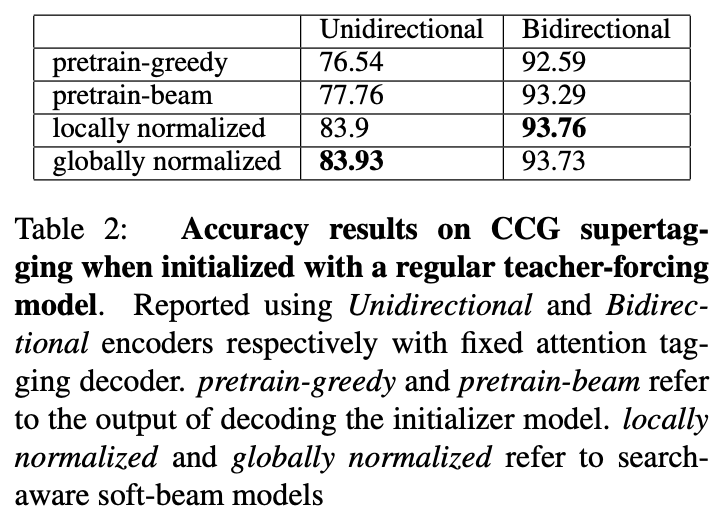
\includegraphics[scale=0.3]{figures/global-local-paper}
    \end{figure}
\end{frame}

\end{document}
